\documentclass[border=2mm]{standalone}
\usepackage{pgfplots}
\usepgfplotslibrary{smithchart}    
\usepgfplotslibrary{polar}   
\usepackage{siunitx} 
\pgfplotsset{compat=1.13}

\begin{document}

    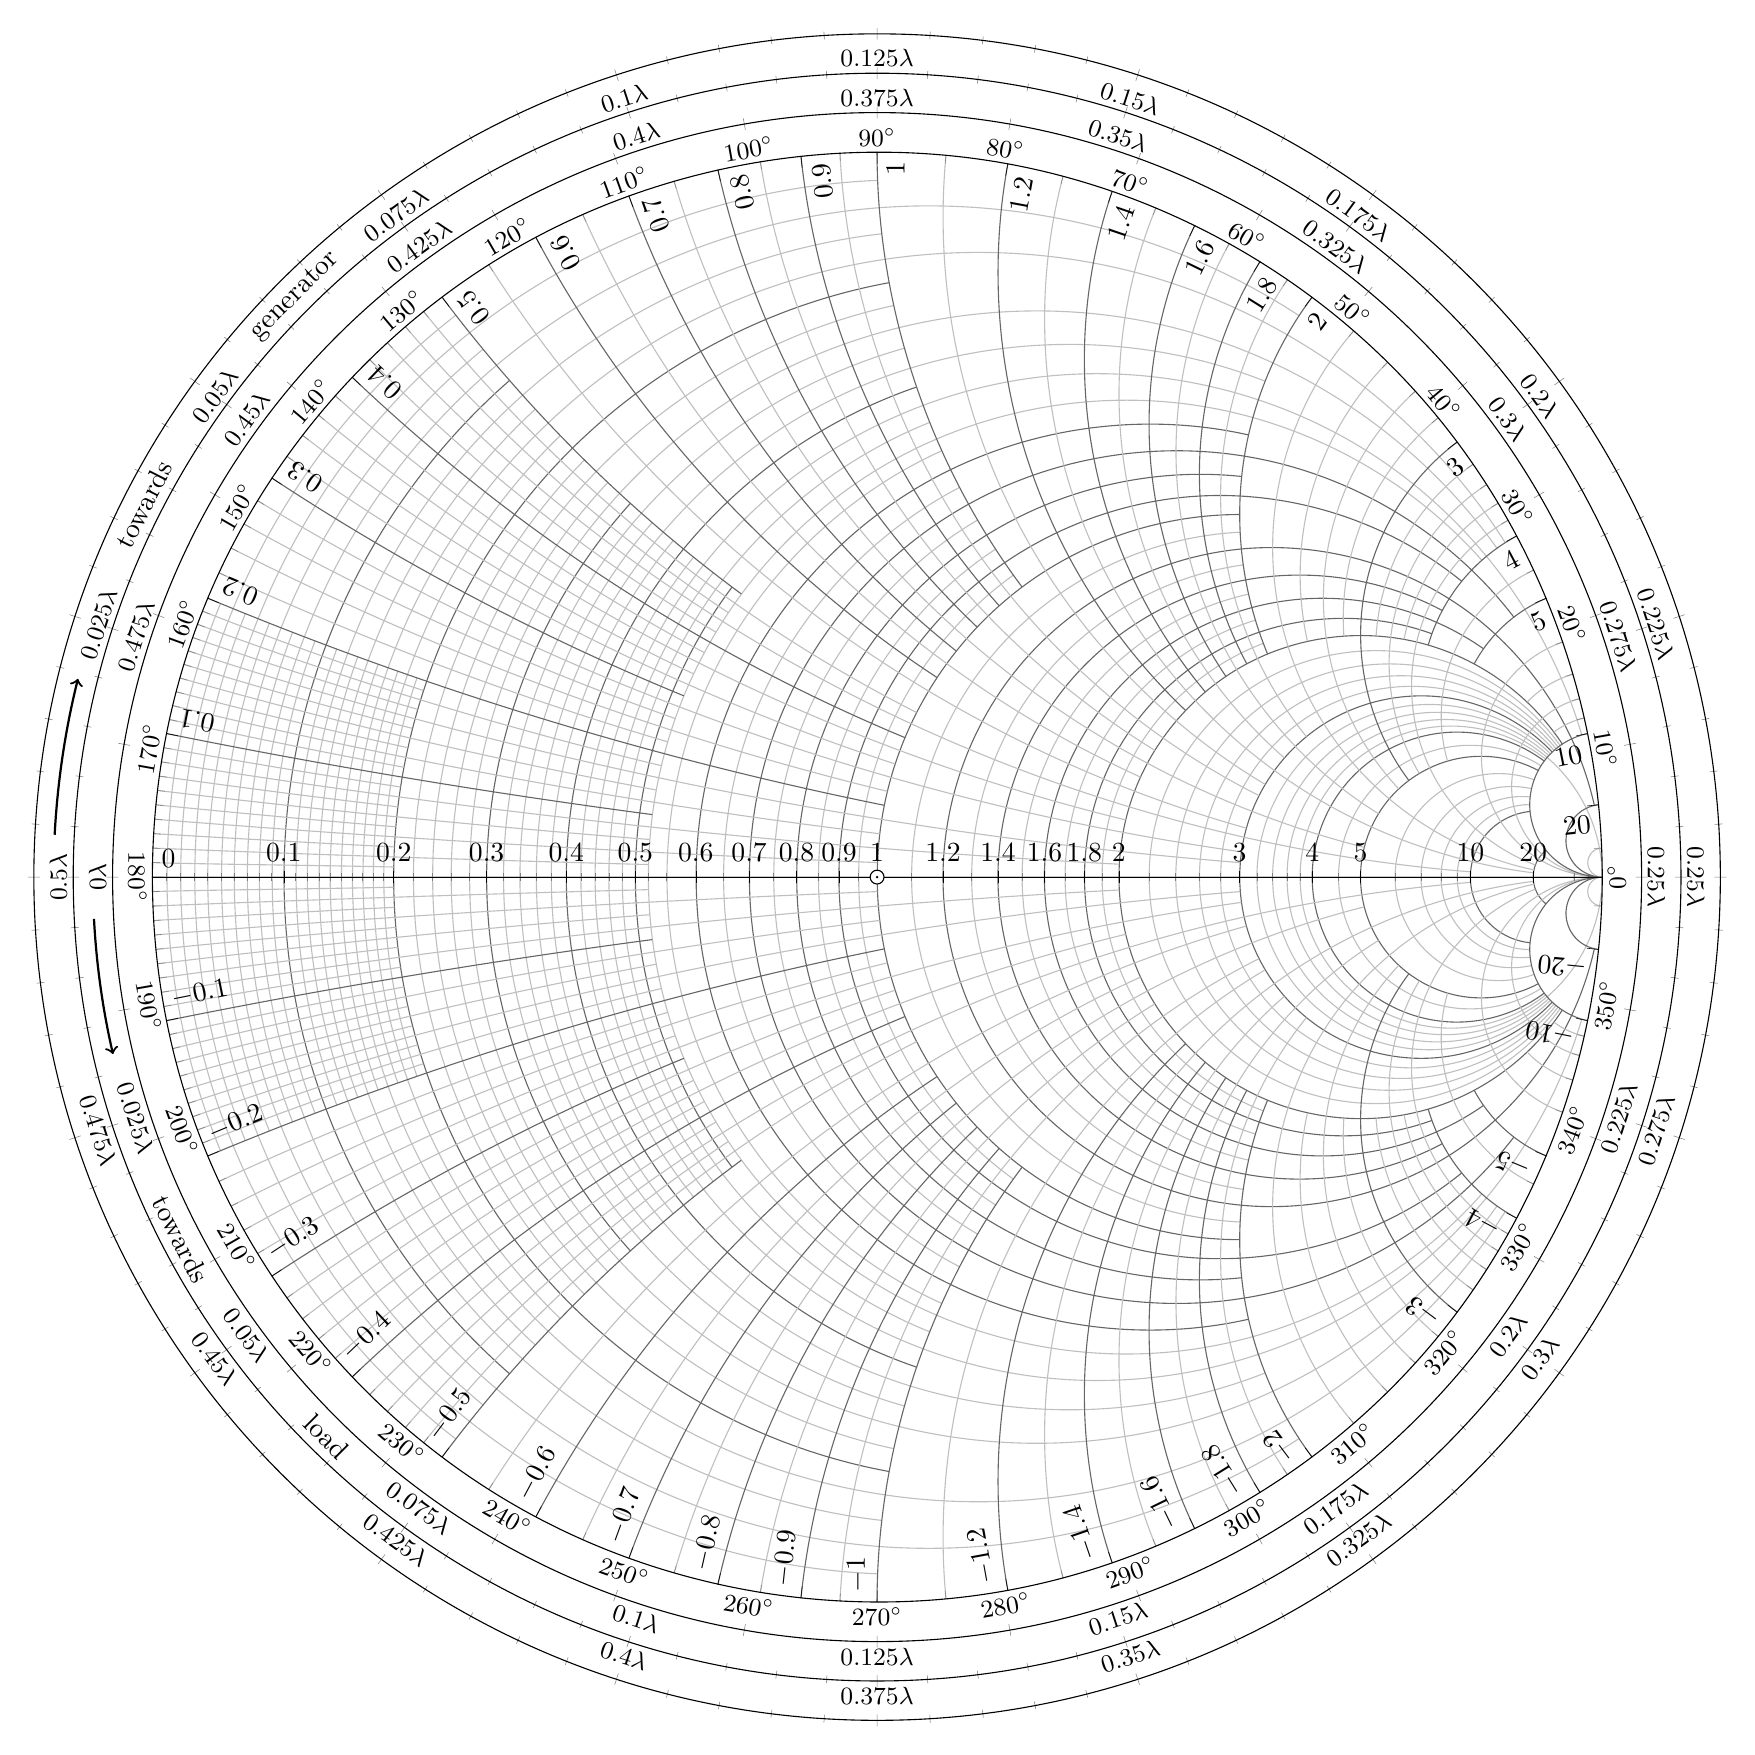
\begin{tikzpicture}
      \pgfmathsetmacro{\xoffset}{10.45*(1-cos(3))-1.25}  
      \pgfmathsetmacro{\yoffset}{sin(3)*10.45+9.2}  
      \draw[,thick,->] (+\xoffset,\yoffset) arc [radius=10.45cm,start angle=177,end angle=166];
      \pgfmathsetmacro{\xoffset}{10.45*(1-cos(18))-1.25}  
      \pgfmathsetmacro{\yoffset}{sin(18)*10.45+9.2} 
      \draw[,draw=none] (+\xoffset,\yoffset) arc [radius=10.45cm,start angle=162,end angle=144] node[midway,sloped]{towards};
      \pgfmathsetmacro{\xoffset}{10.45*(1-cos(36))-1.25}  
      \pgfmathsetmacro{\yoffset}{sin(36)*10.45+9.2} 
      \draw[,draw=none] (+\xoffset,\yoffset) arc [radius=10.45cm,start angle=144,end angle=126] node[midway,sloped]{generator};

      \pgfmathsetmacro{\xoffset}{9.95*(1-cos(-3))-0.75}  
      \pgfmathsetmacro{\yoffset}{sin(-3)*9.95+9.2} 
      \draw[,thick,->] (\xoffset,\yoffset) arc [radius=9.95cm,start angle=183,end angle=193] ;
      \pgfmathsetmacro{\xoffset}{9.95*(1-cos(-18))-0.75}  
      \pgfmathsetmacro{\yoffset}{sin(-18)*9.95+9.2} 
      \draw[,draw=none] (+\xoffset,\yoffset) arc [radius=10.45cm,start angle=198,end angle=216] node[midway,sloped]{towards};
      \pgfmathsetmacro{\xoffset}{9.95*(1-cos(-36))-0.75}  
      \pgfmathsetmacro{\yoffset}{sin(-36)*9.95+9.2} 
      \draw[,draw=none] (+\xoffset,\yoffset) arc [radius=10.45cm,start angle=216,end angle=234] node[midway,sloped]{load};


    \begin{polaraxis}[
                      rotate=180,
                      width=23cm,
                      xshift=1.5cm, 
                      yshift=1.5cm,
                      %xticklabels={$0\lambda$,$0.05\lambda$,$0.1\lambda$,$0.15\lambda$,$0.2\lambda$,$0.25\lambda$},
                      xticklabel style={
                          sloped like x axis={%
                              execute for upside down={\tikzset{anchor=south}},
                              reset nontranslations=false
                          },
                          anchor=north,
                      },
                      xticklabel={\small\pgfmathparse{0.5-\tick/720}\pgfmathprintnumber[fixed,precision=3]{\pgfmathresult}$\lambda$},
                      xtick align=center,
                      xtick={0,18,...,360},
                      grid=none,
                      axis y line = none,
                      minor x tick num={4},
                      ymax=1,
                     ]   
   \end{polaraxis}

    \begin{polaraxis}[
                      rotate=180,
                      width=22cm,
                      xshift=1cm, 
                      yshift=1cm,
                      %xticklabels={$0\lambda$,$0.05\lambda$,$0.1\lambda$,$0.15\lambda$,$0.2\lambda$,$0.25\lambda$},
                      xticklabel style={
                          sloped like x axis={%
                              execute for upside down={\tikzset{anchor=south}},
                              reset nontranslations=false
                          },
                          anchor=north,
                      },
                      xticklabel={\small\pgfmathparse{\tick/720}\pgfmathprintnumber[fixed,precision=3]{\pgfmathresult}$\lambda$},
                      xtick align=center,
                      xtick={0,18,...,360},
                      grid=none,
                      axis y line = none,
                      minor x tick num={4},
                      ymax=1,
                     ]    

    \end{polaraxis}



    \begin{polaraxis}[
                      width=21cm,
                      xshift=-0.5cm, 
                      yshift=-0.5cm,
                      %xticklabels={$0\lambda$,$0.05\lambda$,$0.1\lambda$,$0.15\lambda$,$0.2\lambda$,$0.25\lambda$},
                      xticklabel style={
                          sloped like x axis={%
                              execute for upside down={\tikzset{anchor=north}},
                              reset nontranslations=false
                          },
                          anchor=south,
                      },
                      xticklabel={\small\pgfmathprintnumber{\tick}\si{\degree}},
                      xtick align=center,
                      grid=none,
                      axis y line = none,
                     ]    
   \end{polaraxis}

   \begin{smithchart}[
                      show origin,
                      width=20cm,
                     ]
%    \addplot[mark=none,line width=2]
%        coordinates{
%            (1, 0) (1, 0.1) (1,0.2) (1,0.3) (1,0.4) (1,0.5) (1,0.5)
%        };
%    \addplot[mark=none,line width=0.5]
%        coordinates{
%            (1, 0) (-0.3, 0)  % this one is not drawn outside!!!
%        };
   \end{smithchart}
   \end{tikzpicture} 


\end{document}